% System overview figure. Build from this directory, then include the PDF in the paper:
%   python make_waveforms.py --para-root <path to Para>   # only if the assets change
%   lualatex overview.tex
%   \includegraphics[width=\linewidth]{figures/overview.pdf}
% The waveforms in panel (a) are real: one pilot row (see make_waveforms.py). Panel (b)'s
% waveforms are illustrative. LuaLaTeX because the Vietnamese text needs a font with
% Vietnamese glyphs; TeX Gyre Termes is a Times clone, matching the ICLR body font.

% No EPS images here; skipping epstopdf avoids its grfext dependency on minimal installs.
\expandafter\def\csname ver@epstopdf-base.sty\endcsname{2099/01/01}
\documentclass{article}
\usepackage{graphicx}
\usepackage{tikz}
\usepackage[active,tightpage]{preview}
\PreviewEnvironment{tikzpicture}
\setlength\PreviewBorder{2pt}
\usepackage{fontspec}
\setmainfont{texgyretermes}[Extension=.otf, UprightFont=*-regular, BoldFont=*-bold,
  ItalicFont=*-italic, BoldItalicFont=*-bolditalic]
\usetikzlibrary{positioning,arrows.meta,fit,backgrounds,calc,shapes.geometric,shapes.callouts,
  decorations.pathreplacing}

% Generated by make_waveforms.py from tXO46Ys-7Qc_00028; fractions of each strip's width.
\def\slotA{0.2826}
\def\slotAw{0.1087}
\def\slotB{0.7935}
\def\slotBw{0.1739}
\def\insA{0.2354}
\def\insB{0.4023}


% Draw the tag load balancer on the tagging step. Off until it is implemented.
\newif\ifbalancer
\balancerfalse

\definecolor{speech}{HTML}{3B6EA5}
\definecolor{event}{HTML}{C55A11}
\definecolor{llmfill}{HTML}{ECE4F7}\definecolor{llmline}{HTML}{6A4C93}
\definecolor{modfill}{HTML}{E2F0D9}\definecolor{modline}{HTML}{548235}
\definecolor{grayfill}{HTML}{EDEDED}\definecolor{grayline}{HTML}{7F7F7F}

\begin{document}
\begin{tikzpicture}[
    font=\fontsize{7}{8.4}\selectfont,
    arr/.style={-{Stealth[length=4pt,width=3.2pt]}, line width=0.65pt, black!70},
    feed/.style={-{Stealth[length=3.2pt,width=2.6pt]}, line width=0.45pt, black!45},
    steptxt/.style={font=\fontsize{7.2}{8.6}\selectfont\bfseries, inner sep=1pt},
    num/.style={circle, fill=black!75, text=white, inner sep=0pt, minimum size=8pt,
                font=\fontsize{5.5}{5.5}\selectfont\bfseries},
    small/.style={font=\fontsize{6}{7.2}\selectfont, text=black!70, inner sep=1pt},
    lab/.style={font=\fontsize{6}{7}\selectfont\itshape, text=black!65, inner sep=1pt},
    panel/.style={draw=black!25, rounded corners=4pt, inner sep=5pt},
    ptitle/.style={font=\fontsize{7.5}{9}\selectfont\bfseries, anchor=north west,
                   inner sep=3pt},
    img/.style={inner sep=0pt, outer sep=1pt},
    % Model icon: three stacked layers.
    layers/.pic={
      \foreach \o in {0.16, 0.08, 0} {
        \filldraw[fill=#1fill, draw=#1line, rounded corners=1.5pt, line width=0.6pt]
          (-0.55+\o, -0.35+\o) rectangle (0.45+\o, 0.25+\o);
      }
      \foreach \yy in {-0.17, -0.05, 0.07}
        \draw[#1line, line width=0.5pt] (-0.4, \yy) -- (0.3, \yy);
    },
    % Database icon.
    db/.style={cylinder, shape border rotate=90, aspect=0.3, draw=grayline,
               fill=grayfill, minimum width=0.9cm, minimum height=0.85cm, line width=0.6pt},
  ]
  \newcommand{\steplabel}[3]{%
    \node[steptxt, anchor=north] (tmp) at #1 {#3};
    \node[num, left=2pt of tmp] {#2};}

  % ═══ (a) Training-data synthesis ═══════════════════════════════════════════════
  % ── (1) Slot finding: real pauses between aligned words ──
  \node[img] (src) at (2.3, 0.15)
    {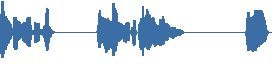
\includegraphics[width=4.6cm, height=1.1cm]{assets/source.pdf}};
  \begin{scope}[on background layer]
    \foreach \c/\w in {\slotA/\slotAw, \slotB/\slotBw}
      \fill[black!10] ($(src.south west)+({(\c-\w/2)*4.6}, 0)$)
        rectangle ($(src.north west)+({(\c+\w/2)*4.6}, 0)$);
  \end{scope}
  \node[num, fill=event] at ($(src.north west)+({\slotA*4.6}, 0.15)$) {1};
  \node[num, fill=white, draw=black!75, text=black!75]
    at ($(src.north west)+({\slotB*4.6}, 0.15)$) {2};
  \node[small, below=1pt of src]
    {…chứ thôi , {\color{event}\textbf{<1>}} để nó lành thôi … \textbf{<2>} nhưng mà…};
  \steplabel{(2.3, -1.0)}{1}{Slot finding}

  % ── (2) Tag selection: an omni LLM listens and picks one slot + one tag ──
  \begin{scope}[shift={(6.25, 0.15)}]
    \filldraw[fill=llmfill, draw=llmline, rounded corners=3pt, line width=0.7pt]
      (-0.6, -0.5) rectangle (0.6, 0.5);
    \foreach \a in {-0.25, 0, 0.25} \foreach \b in {-0.12, 0.12}
      \draw[llmline!70, line width=0.35pt] (-0.32, \a) -- (0, \b);
    \foreach \b in {-0.12, 0.12}
      \draw[llmline!70, line width=0.35pt] (0, \b) -- (0.32, 0);
    \foreach \a in {-0.25, 0, 0.25} \fill[llmline] (-0.32, \a) circle (1.6pt);
    \foreach \b in {-0.12, 0.12} \fill[llmline] (0, \b) circle (1.6pt);
    \fill[llmline] (0.32, 0) circle (1.8pt);
    \coordinate (llm) at (0, 0);
  \end{scope}
  \node[small, below=0.55cm of llm] {Qwen3-Omni};
  \steplabel{(6.25, -1.0)}{2}{Tag selection}
  \draw[arr] (src.east) -- node[lab, above] {audio +} node[lab, below] {slots}
    ($(llm)+(-0.62, 0)$);

  \ifbalancer
    \draw[feed] ($(llm)+(-0.3, 0.5)$) to[out=110, in=70, looseness=4]
      node[lab, above] {tag balancer} ($(llm)+(0.3, 0.5)$);
  \fi

  % ── (3) Clip selection: weighted sampling among clips of the chosen class ──
  \foreach \i/\yy/\p in {0/0.6/0.62, 1/0.15/0.24, 2/-0.3/0.14} {
    \node[img] (c\i) at (9.35, \yy)
      {\includegraphics[width=1.5cm, height=0.42cm]{assets/cand\i.pdf}};
    \fill[event!70] ($(c\i.east)+(0.12, -0.07)$) rectangle ++({\p*1.3}, 0.14);
  }
  \draw[event, line width=0.7pt, rounded corners=2pt]
    ($(c0.south west)+(-0.06, -0.02)$) rectangle ($(c0.north east)+(0.06+0.95, 0.02)$);
  \node[small, above=1pt of c0.north east, xshift=0.5cm] {$p\propto e^{-\Sigma\lambda d}$};
  \steplabel{(9.75, -1.0)}{3}{Clip selection}
  \draw[arr] ($(llm)+(0.62, 0)$) -- node[lab, above] {<1>}
    node[lab, below, text=event] {[laughter]} ($(c1.west)+(-0.05, 0)$);

  \node[db] (corpus) at (12.75, 0.15) {};
  \node[small, below=1pt of corpus] {NVV clips};
  \draw[arr] (corpus.west) -- ($(c1.east)+(1.0, 0)$);

  % ── (4) Voice conversion into the host speaker's voice ──
  \node[img] (vin) at (0.85, -2.65)
    {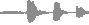
\includegraphics[width=1.5cm, height=0.42cm]{assets/cand0.pdf}};
  \begin{scope}[shift={(2.45, -2.65)}]
    \filldraw[fill=event!12, draw=event, line width=0.7pt] (0, 0) circle (0.36);
    \draw[event, line width=0.8pt, -{Stealth[length=3pt]}] (100:0.2) arc (100:330:0.2);
    \draw[speech, line width=0.8pt, -{Stealth[length=3pt]}] (-80:0.2) arc (-80:150:0.2);
    \coordinate (vc) at (0, 0);
  \end{scope}
  \node[img] (vout) at (4.05, -2.65)
    {
\includegraphics[width=1.5cm, height=0.42cm]{assets/converted.pdf}};
  \draw[arr] (vin.east) -- ($(vc)+(-0.38, 0)$);
  \draw[arr] ($(vc)+(0.38, 0)$) -- (vout.west);
  \node[small, above=0.38cm of vc] {Seed-VC};
  \node[lab, below=0.36cm of vc, text=speech] {into the host speaker's voice};
  \steplabel{(2.45, -3.62)}{4}{Voice conversion}

  % The selected clip comes down from (3) into (4).
  % Leaves from the right of the candidates so it clears the "Clip selection" label.
  \draw[arr] ($(c2.south east)+(1.15, -0.05)$) -- ++(0, -0.82) -| (vin.north);

  % ── (5) Splicing: the event goes into the chosen pause ──
  \node[img] (sp) at (7.3, -2.65)
    {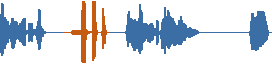
\includegraphics[width=4.6cm, height=1.1cm]{assets/spliced.pdf}};
  \draw[decorate, decoration={brace, amplitude=3pt}, event, line width=0.6pt]
    ($(sp.north west)+({\insA*4.6}, 0.03)$) -- ($(sp.north west)+({\insB*4.6}, 0.03)$)
    node[midway, above=2pt, font=\fontsize{6}{7}\selectfont\bfseries] {[laughter]};
  \node[small, below=1pt of sp]
    {…chứ thôi , {\color{event}\textbf{[laughter]}} để nó lành thôi…};
  \steplabel{(7.3, -3.62)}{5}{Splicing}
  \draw[arr] (vout.east) -- (sp.west);

  % ── (6) Quality filter ──
  \begin{scope}[shift={(10.45, -2.65)}]
    \filldraw[fill=grayfill, draw=grayline, line width=0.7pt, rounded corners=0.5pt]
      (-0.4, 0.35) -- (0.4, 0.35) -- (0.1, -0.05) -- (0.1, -0.35) -- (-0.1, -0.25)
      -- (-0.1, -0.05) -- cycle;
    \draw[modline, line width=1.4pt] (0.22, -0.2) -- (0.32, -0.32) -- (0.52, -0.02);
    \coordinate (qf) at (0, 0);
  \end{scope}
  \node[small, above=0.38cm of qf] {NISQA};
  \steplabel{(10.45, -3.62)}{6}{Filter}
  \draw[arr] (sp.east) -- ($(qf)+(-0.42, 0)$);

  % ── Output dataset ──
  \node[db] (data) at (12.75, -2.65) {};
  \node[steptxt, anchor=north, align=center] at (12.75, -3.3) {Synthetic\\NVV data};
  \draw[arr] ($(qf)+(0.42, 0)$) -- (data.west);

  \begin{scope}[on background layer]
    \node[panel, fit={(0, 1.3) (13.6, -4.1)}, yshift=4pt] (PA) {};
  \end{scope}
  \node[ptitle] at (PA.north west) {(a) Training-data synthesis};

  % ═══ (b) Fine-tuning and inference ═════════════════════════════════════════════
  \def\yb{-6.0}
  % Training: pretrained -> fine-tuned on the synthetic data plus untagged speech.
  \pic at (1.0, \yb) {layers=gray};
  \node[steptxt, anchor=north] at (1.0, \yb-0.62) {OmniVoice};
  \node[small, anchor=north] at (1.0, \yb-0.9) {pretrained};
  \node[db, minimum width=0.7cm, minimum height=0.6cm] at (3.3, \yb+0.42) {};
  \node[small, anchor=north] at (3.3, \yb-0.08) {NVV data + ViVoice};
  \draw[arr] (1.75, \yb) -- node[lab, below=8pt] {fine-tune} (4.95, \yb);
  \pic at (5.75, \yb) {layers=mod};
  \node[steptxt, anchor=north] at (5.75, \yb-0.62) {OmniVoice};
  \node[small, anchor=north] at (5.75, \yb-0.9) {fine-tuned};

  \draw[black!25, dashed, line width=0.6pt] (7.05, \yb+1.05) -- (7.05, \yb-1.15);

  % Inference: tagged text + a reference voice in, speech with the NVV out.
  \node[draw=grayline, fill=white, rounded corners=2pt, inner sep=3pt,
        font=\fontsize{6.2}{7.2}\selectfont] (prompt) at (8.6, \yb+0.32)
    {hôm nay vui quá {\color{event}\textbf{[laughter]}} …};
  \node[img] (ref) at (8.6, \yb-0.42)
    {
\includegraphics[width=1.7cm, height=0.45cm]{assets/reference.pdf}};
  \node[small, below=0pt of ref] {reference voice};
  \pic at (10.75, \yb) {layers=mod};
  \node[small, anchor=north] at (10.75, \yb-0.45) {fine-tuned};
  \draw[arr] (prompt.east) -- (10.1, \yb+0.1);
  \draw[arr] (ref.east) -- (10.1, \yb-0.18);
  \node[img] (gen) at (12.65, \yb)
    {
\includegraphics[width=1.8cm, height=0.55cm]{assets/generated.pdf}};
  \node[small, below=1pt of gen] {speech with the NVV};
  \draw[arr] (11.45, \yb) -- (gen.west);

  \begin{scope}[on background layer]
    \node[panel, fit={(0, \yb+1.2) (13.6, \yb-1.25)}, yshift=4pt] (PB) {};
  \end{scope}
  \node[ptitle] at (PB.north west) {(b) Fine-tuning and inference};
\end{tikzpicture}
\end{document}
